% \documentclass{report}
% 
% \usepackage{fancyhdr}
\usepackage{fourier-orns}
\usepackage{hyperref}%% To refrence links / jumps
\usepackage{chngcntr} %% For some extra counters numberings
\usepackage[a4paper, right = 0.5in, left = 0.5in,top = 1in , bottom = 1in]{geometry}
\usepackage{etoolbox} %% Provides like a language for advanced customization
\usepackage{datetime} %% For dates of course
\usepackage{lastpage} %% provides pages numbers
\usepackage[sc]{titlesec} %% modify titles
\usepackage{enumerate}
\usepackage{cancel}
\usepackage{tikzsymbols}
\usepackage[dvipsnames]{xcolor}
\usepackage{import}
\usepackage{pdfpages} %% include other pdfs
\usepackage{transparent} %% Transparency
\usepackage{xcolor}  %% Colors
\usepackage[many]{tcolorbox}
\usepackage[framemethod=TikZ]{mdframed}
\usepackage{amsmath,amsfonts,amsthm,amssymb,mathtools}
\usepackage{tikz}
\usepackage{bookmark}
\usepackage{graphicx}
\usepackage{mathpazo}

\usepackage{fontawesome5}

\linespread{1.5}


\titleformat{\chapter}[display]   
{\fontfamily{ppl}\selectfont\huge\color{YellowOrange!80!orange}} % Font style and size 
{\raggedleft\color{purple}\fontsize{70}{0pt}\selectfont\thechapter}   
{-1.5cm}    			                          % Space between the chapter number and title
{
	\begin{tikzpicture}[overlay]
		\node[anchor = west,yshift = 0.2cm,xshift = -1cm] {\fontsize{90}{20} $\int_{}^{} $};
		\node[yshift = 4cm, xshift = 17cm]   {\includegraphics[width = 4cm]{preview0}};
	\end{tikzpicture}
\hspace{1cm}\Huge\raggedright\MakeUppercase}

\titleformat{\section}[block]
{
\fontfamily{ppl}\selectfont\huge\color{YellowOrange!80!orange}
}
{
\color{purple}\fontsize{20}{0pt}\selectfont\thesection 
}
{0cm}
{
	\begin{tikzpicture}[overlay]
		\node[anchor = west,yshift = 0.2cm,xshift = -0.4cm, circle = 1pt] {};
	\end{tikzpicture}
}

\titlespacing*{\section}{0pt}{0.7cm}{1.5cm}


\newcommand{\divider}
{
	\begin{center}
	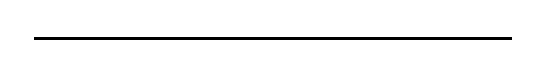
\begin{tikzpicture}
		\draw[thick, black] (0.25*\textwidth, 0) -- (0.75*\textwidth, 0);
		\node[rotate = 360 - 90, xshift = -0.6pt, yshift = 1pt] at (0.25*\textwidth,0){\decotwo};
		\node[rotate = 90, xshift = -0.6pt, yshift = 1pt] at (0.75*\textwidth,0){\decotwo};
	\end{tikzpicture}
	\end{center}
}

\pagestyle{fancy}

\newcommand{\lecday}[1][]
{
    \def\datee{#1}
    \fancyhead[L]{\datee}
}



\newcommand{\signature}
{
	\begin{tikzpicture}[remember picture,overlay]
		\node[fill = YellowOrange!20!white] at ([yshift = 1cm, xshift = -3cm]current page.south east) {\fontsize{10pt}{0pt}{\itshape Kara.$\mathcal{A}$}};
	\end{tikzpicture}
}

\AddToHook{shipout/background}{
  \begin{tikzpicture}[remember picture, overlay]
	  \node[] at ([yshift = 1.5cm,xshift = \textwidth /2 + 0.9cm]current page.south west) {\includegraphics[width = 0.5cm]{preview3}};
	  \node[] at ([yshift = 1.5cm,xshift = - \textwidth /2 - 0.9cm]current page.south east) {\includegraphics[width = 0.5cm]{preview4}};
  \end{tikzpicture}
}



\newtcolorbox[auto counter, number within = section]{remark}[1][]
{
       		title = Remark #1,
		enhanced,
		boxrule = 0pt,
		colback = white,
		breakable,
		arc = 4pt,
		colbacktitle = cyan,
		colback = cyan!5!white,
		segmentation style =
		{
			solid,cyan,thick,
		},
		attach boxed title to top left =
		{
			xshift = 0cm,
		},
		boxed title style =
		{
			boxrule = 0pt,
			sharp corners,
			drop fuzzy shadow = {cyan},
		},
		drop fuzzy shadow = {cyan!80!black},
}

\newtcolorbox[auto counter, number within = section]{theorem}[1][]
{                                      
		title = Theorem \thetcbcounter : #1,
		enhanced, 
		boxrule = 0pt,
		colback = white,
		breakable,
		arc = 4pt,
		colbacktitle = purple,
		colback = purple!5!white,
		segmentation style = 
		{
			solid, purple,thick,
		},
		attach boxed title to top left = 
		{
			xshift = 0cm, 
		},
		boxed title style = 
		{
			boxrule = 0pt,
			sharp corners,
			drop fuzzy shadow = {purple},
		},
		drop fuzzy shadow = {purple!80!black},
}

\newtcolorbox[auto counter, number within = section]{definition}[1][]
{                                      
		title = Definition \thetcbcounter : #1,
		enhanced, 
		boxrule = 0pt,
		colback = white,
		arc = 4pt,
		breakable,
		colbacktitle = YellowOrange!80!black,
		segmentation style = 
		{
			solid, YellowOrange,thick,
		},
		attach boxed title to top left = 
		{
			xshift = 0cm, 
		},
		colback = YellowOrange!5!white,
		boxed title style = 
		{
			boxrule = 0pt,
			sharp corners,
			drop fuzzy shadow = {YellowOrange!80!orange},
		},
		drop fuzzy shadow = {YellowOrange!80!black},
}

\newtcolorbox[auto counter, number within = section]{corollary}[1][]
{                                      
		title = corollary \thetcbcounter : #1,
		enhanced, 
		boxrule = 0pt,
		colback = white,
		arc = 4pt,
		breakable,
		colbacktitle = YellowOrange!80!black,
		segmentation style = 
		{
			solid, YellowOrange,thick,
		},
		attach boxed title to top left = 
		{
			xshift = 0cm, 
		},
		colback = YellowOrange!5!white,
		boxed title style = 
		{
			boxrule = 0pt,
			sharp corners,
			drop fuzzy shadow = {YellowOrange!80!orange},
		},
		drop fuzzy shadow = {YellowOrange!80!black},
}


\newtcolorbox{example}[1][]
{                                      
		title = Example,
		enhanced, 
		boxrule = 0pt,
		colback = white,
		arc = 4pt,
		segmentation style = 
		{
			solid, SpringGreen,thick,
		},
		breakable,
		colback = SpringGreen!5!white,
		colbacktitle = SpringGreen!80!black,
		attach boxed title to top left = 
		{
			xshift = 0cm, 
		},
		boxed title style = 
		{
			boxrule = 0pt,
			sharp corners,
			drop fuzzy shadow = {SpringGreen!80!orange},
		},
		drop fuzzy shadow = {SpringGreen!80!black},
}


\newcommand{\integral}[4]{\int\limits_{#1}^{#2} #4 d#3}
\newcommand{\limit}[3]{\lim\limits_{#1 \rightarrow #2} #3}
\newcommand{\strone}[2]{\left[ \begin{gathered}#1\\ #2\end{gathered} \right] }
\newcommand{\strtwo}[2]{\left\{ \begin{gathered}#1\\ #2\end{gathered} \right\} }
\newcommand{\strthree}[2]{\left\lfloor \begin{gathered}#1\\ #2\end{gathered} \right\rfloor }


\newcommand{\startbf}[1]{\text{\bfseries{#1}}}
\newcommand{\sett}[1]{\left\{ #1 \right\}}
\newcommand{\thesis}[1]{\left( #1 \right)}
\newcommand{\brkt}[1]{\left[ #1 \right]}
\newcommand{\floor}[1]{\left\lfloor #1 \right\rfloor}


\DeclareMathOperator{\img}{im} % Image
\DeclareMathOperator{\Img}{Im} % Image
\DeclareMathOperator{\coker}{coker} % Cokernel
\DeclareMathOperator{\Coker}{Coker} % Cokernel
\DeclareMathOperator{\Ker}{Ker} % Kernel
\DeclareMathOperator{\rank}{rank}
\DeclareMathOperator{\Spec}{Spec} % spectrum
\DeclareMathOperator{\Tr}{Tr} % trace
\DeclareMathOperator{\pr}{pr} % projection
\DeclareMathOperator{\ext}{ext} % extension
\DeclareMathOperator{\pred}{pred} % predecessor
\DeclareMathOperator{\dom}{dom} % domain
\DeclareMathOperator{\ran}{ran} % range
\DeclareMathOperator{\Hom}{Hom} % homomorphism
\DeclareMathOperator{\Mor}{Mor} % morphisms
\DeclareMathOperator{\End}{End} % endomorphism


\newcommand{\lm}{\ensuremath{\lambda}}
\newcommand{\eps}{\ensuremath{\epsilon}}
\newcommand{\veps}{\ensuremath{\varepsilon}}
\newcommand{\al}{\ensuremath{\alpha}}
\newcommand{\bb}{\ensuremath{\beta}}
\newcommand{\cc}{\ensuremath{\gamma}}
\newcommand{\dd}{\ensuremath{\delta}}
\newcommand{\DD}{\ensuremath{\Delta}}
\newcommand{\ff}{\ensuremath{\phi}}
\newcommand{\FF}{\ensuremath{\varphi}}

\newcommand{\RR}{\mathbb{R}}
\newcommand{\RO}{\mathcal{R}}
\newcommand{\EE}{\mathbb{E}}
\newcommand{\CC}{\mathbb{C}}
\newcommand{\RW}{\mathbb{R}^2}
\newcommand{\RT}{\mathbb{R}^3}
\newcommand{\RN}{\mathbb{R}^n}
\newcommand{\DS}{\mathcal{D}}

\newcommand{\KK}{\mathbb{K}}
\newcommand{\KW}{\mathbb{K}^2}
\newcommand{\KT}{\mathbb{K}^3}
\newcommand{\KN}{\mathbb{K}^n}

\newcommand{\NN}{\mathbb{N}}

\newcommand{\PS}{\mathcal{P}}
\newcommand{\AS}{\mathcal{E}}
\newcommand{\FS}{\mathcal{F}}
\newcommand{\LS}{\mathcal{L}}
\newcommand{\MS}{\mathcal{M}}


















\lecday[2025-05-22]

% \begin{document}

\begin{proof}
Take $\KK = \CC  $ (the general case), the statement of the proposition
is trivial for $x = 0_{E} $ or $y = 0_{E} $. Suppose for 
the sequel that $x \neq 0_{E} $  and $y \neq 0_{E} $. Consider
the unitary vector of $E $ : 
\[
u := \frac{x}{\| x \| _{E}} \quad 
\text{ and } \quad 
v := \frac{y}{\| y \| _{E}}  \quad \text{ so $\| u \|_{E} = \| v \|_{E} =1 $ } 
\]
Since $\left\langle , \right\rangle $ is Positive Definite, we have : 
\[
\left\langle 
  u - \overline{\left\langle u,v \right\rangle } v, 
  u - \overline{\left\langle u,v \right\rangle } v
\right\rangle  \geq 0
\]
and 
\begin{align*}
\left\langle u - \overline{\left\langle u,v \right\rangle } v,
u - \overline{\left\langle u,v \right\rangle } v\right\rangle  &= 0 \\
\iff \quad \quad \quad \quad  u - \overline{\left\langle u,v \right\rangle } v &= 0_{E} \quad 
\quad  \quad (*)  
\end{align*}
which implies that $u,v $ are collinear. \\
On the other hand, by expanding the inner product 
$
\left\langle 
  u-\overline{\left\langle u,v \right\rangle } v, 
  u- \overline{\left\langle u,v \right\rangle } v
\right\rangle$
using the sesquilinearity and the hermitian symmetry 
of $\left\langle . , . \right\rangle  $, we get : 
\begin{align*}
\left\langle u - \overline{\left\langle u,v \right\rangle } v, 
u - \overline{\left\langle u,v \right\rangle } v \right\rangle  &= 
\underbrace{
\left\langle u,u \right\rangle
}_{\| u \| ^2  = 1} 
- \overline{\left\langle u,v \right\rangle } 
\left\langle u,v \right\rangle  - 
\left\langle u,v \right\rangle  \left\langle  v,u \right\rangle  + 
\left\langle u,v \right\rangle  \overline{\left\langle u,v \right\rangle } 
\underbrace{
\left\langle v,v \right\rangle 
}_{ \| v \| ^2  = 1} 
\\
                                                                &= 
                                                                1 - \left| 
                                                                \left\langle u,v \right\rangle 
                                                                \right|^2 
\end{align*}
By inserting this in $(*)$, we derive that : 
\begin{align*}
&\begin{cases}
 \left| \left\langle u,v \right\rangle  \right| \leq  1
 \\
 \left| \left\langle u,v \right\rangle  \right| = 1 \iff 
 \text{ $u $ and $v $ are collinear }  
\end{cases}
\\
  &\begin{cases}
  \left| \left\langle \frac{x}{\| x \| }, 
  \frac{y}{\| y \| }\right\rangle  \right| \leq 1 
  \iff  \left| \left\langle x,y \right\rangle  \right| \leq 
  \| x \| \| y \|  \\
  \left| \left\langle \frac{x}{\| x \| }, 
  \frac{y}{\| y \| }\right\rangle  \right| = 1  
  \iff x \text{ and } y \text{ are collinear } 
  \end{cases}
\end{align*} 
That is : 
\[
\begin{cases}
  \left| \left\langle x,y \right\rangle  \right| \leq 
  \| x \| \cdot  \| y \|  \\
  \text{           and } 

  \\
  \left| \left\langle x,y \right\rangle  \right| = 
  \| x \|  \cdot  \| y \|  \iff 
  x \text{ and } y \text{ are collinear } 
\end{cases}
\]
The proposition is proved.
\end{proof}

\begin{corollary}[(The Triangle Inequality)]
  Let $\KK = \RR $  or $\CC  $ and $E $ be a $\KK $-vector space equipped
  with an inner product $\left\langle \cdot ,\cdot  \right\rangle  $. Let 
  also $\| . \|  $  be the norm associated to $\left\langle \cdot , \cdot  \right\rangle  $. 
  Then we hvae for all $x,y \in  E $ :
  \[
    \fbox{
    $\| x + y \|  \leq \| x \| + \| y \|$
    }
  \]
  \textcolor{blue}{
  It's The Triangular inequality !
  }
\end{corollary}
\begin{proof}
for $\KK = \CC  $ let $x,y \in  E $, we have :
\begin{align*}
  \| x+y \| ^2  &= \left\langle x + y, x + y \right\rangle  \\
                &= \left\langle x, x \right\rangle  + 
                \left\langle x, y \right\rangle + \left\langle y,x \right\rangle  + 
                \left\langle y, y \right\rangle  \\
                &= \| x \| ^2  + \| y \| ^2 + 2 \underbrace{
                \mathcal{R} \left\langle x,y \right\rangle  
                }_{ \leq \left| \left\langle x,y \right\rangle  \right| \overset{
                    \textcolor{blue}{Cauchy-Schawrtz}
                  }{ \leq } 
                \| x \| \| y \| }  
                \\
                &= \| x \| ^2  + \| y \| ^2 + 
                2 \| x \|  \cdot  \| y \| 
                = \left( \| x \| + \| y \|   \right)^2 
\end{align*}
Hence : 
\[
\| x + y \|  \leq \| x \| + \| y \| 
\]
as required.
\end{proof}
\textsc{ \large \underline{Consequence (Immediate ) : \warning}}\\ 
A norm associated to an inner product of a $\KK $-vector space $E$, where 
($\KK = \RR  $ or $\CC  $) is really a norm on $E$. 
\divider
\begin{definition}[]
We call a pre-Hilbert space any vector space over $\RR $ or $\CC  $, equipped 
with an inner product. To clarify, we sometimes use the terminology of
\textcolor{blue}{real pre-Hilbet space} and \textcolor{red}{complex pre-Hilbert space}
\end{definition}
\begin{definition}[]
  We call 
  \textcolor{blue}{
    Hilbet-spcae
  } any pre-Hilbert which is 
  \textcolor{blue}{Banach} with respect to the norm associated to its 
  \underline{inner product}.
\end{definition}
\textsc{\large \underline{Orthogonality in a pre-Hilbert space : \warning }} \\
Let $E $ be a pre-Hilbert space and let $x,y \in  E $, we say 
that $x $ and $y $ are orthogonal (and we write $x \bot y $ ) if :
\[
  \textcolor{blue}{
  \fbox{
    $ \left\langle x,y \right\rangle = 0$
  }
  }
\]
\textsc{\large \underline{Some Important Identities in a pre-Hilbert space : \warning }}\\
Let $E $ be a pre-Hilbert space. 
\\
\textsc{\underline{(1) The Pythagorean Theorem : \lefthand }} \\
For any $x,y \in  E $  with $x \bot y $, we have :
\[
\| x + y \| = \| x \| ^2  + \| y \| ^2 
\]
\underline{\lefthand~ Generalization : } \\
Let $n \in  \NN $ and $x_1, \hdots , x_n  \in  E $, \textcolor{blue}{pairwise} orthogonal 
(i.e. $x_{k} \bot x_{l} $ for $k \neq l $ ), then we have :  
\[
\| x_1 + \hdots + x_n  \| ^2  = 
\| x_1 \| ^2 + \hdots + \| x_n  \| ^2 
\]
\textsc{\underline{(2) The Polarization Formula : \lefthand }} \\
The polarisation formula expresses the inner product in terms of it's
assocaited norm. In the \textcolor{blue}{real} case, for all $x,y \in  E $, we have :
\begin{align*}
  \left\langle x,y \right\rangle &= \frac{1}{2}
\left( \| x+y \| ^2  - \| x \| ^2  - \| y \| ^2  \right) \\
  \left\langle x,y \right\rangle  &= \frac{1}{4}
  \left( \| x+y \| ^2  - \| x-y \| ^2  \right)
\end{align*}
Some additional notes, for the \textcolor{blue}{imaginary} case
\[
  \left\langle x,y \right\rangle  = \mathcal{R} \left\langle x,y \right\rangle + 
  i \mathcal{I} \left\langle x,y \right\rangle 
\]
\begin{align*}
  \left\langle x,y \right\rangle &= 
  \mathcal{R} \left\langle x,y \right\rangle + 
  i \mathcal{I} \left\langle x,y \right\rangle \\
                                 &= \mathcal{R} 
                                 \left\langle x,y \right\rangle - 
                                 i \mathcal{R} \left\langle x, iy\right\rangle   \quad 
                                 \quad \quad 
                                   \textcolor{red}{(\mathcal{I} \omega  = - \mathcal{R} i\omega }
                                 \\
                                 &= \mathcal{R} \left\langle x,y \right\rangle - 
                                 i \mathcal{R} \left\langle x, iy \right\rangle  \\
                                 &= 
                                 \frac{1}{4}
                                 \left( 
                                   \| x+y \| ^2  - 
                                   \| x-y \| ^2 
                                 \right) - 
                                 \frac{1}{4}
                                 \left\langle \| x+iy \| ^2 - 
                                 \| x - iy \| ^2 \right\rangle 
\end{align*}
To formally put it, for all $x,y \in E $, we have : 
\[
\left\langle x,y \right\rangle = 
\frac{1}{4}
\left( 
  \| x+y \| ^2  - \| x-y \| ^2 
\right) - \frac{1}{4} i
\left( 
  \| x+iy \| ^2 - \| x-iy \|^2 
\right)
\]
\textsc{\underline{(3) The Parallelogram Identity : \lefthand }} \\
For every $x,y \in E $, we have : 
\[
  \fbox{
    \textcolor{red}{
    $ \| x+y \| ^2  + \| x-y \| ^2  = 2 \left( \|x  \|^2 + \| y \| ^2   \right) $ 
    }
  }
\]
\begin{center}
\it
"In any parallelogram, the sum of the squares of the lengths of the two diagonals is equal
to the sum of the squares of the lengths of the four sides"
\normalfont
\end{center}
\begin{example}
  Consider $\| . \| _{1} $  in $\RR ^2  $ : 
  \[
  x = 
\begin{pmatrix}
  1 \\
  0 \\
\end{pmatrix} \quad \quad 
  y = 
\begin{pmatrix}
  0 \\
  1 \\
\end{pmatrix}
  \]
  \begin{align*}
    \| x+y \| _{1} &= 
    \| 
\begin{pmatrix}
  1 \\
  1 \\
\end{pmatrix}
    \|  = 2 
    \\
    \| x-y \| _{1} &= 
    \| 
\begin{pmatrix}
  1 \\
  -1 \\
\end{pmatrix}
    \|  = 2 
  \end{align*}
  and $\| x \|_{1} = \| y \| _{1} = 1 $, 
  \[
  \| x+y \| _{1}^2 + \| x-y \| _{1}^2  = 8 
  \large \neq  
  \normalfont 
  4 = 
  2 \left( 
    \| x \| _{1}^2  + \| y \| _{1}^2 
  \right) 
  \]
\end{example}
\begin{theorem}[(p.Jordan \& j.Von Neumann)]
  A N.V.S over $\KK= \RR  $ or $\CC  $ is pre-Hilberrt 
  if and only if it's norm satisfies the \textcolor{blue}{Parallelogram Identity}
\end{theorem}
\begin{proof}
  It's already shown that the 
  \textcolor{blue}{
  Parallelogram identity 
  } is necessary for a N.V.S over ($\RR $ or $\CC  $ ) to be pre-Hilbert.
  Let us show that it is even sufficient we only deal with the case 
  $\KK = \RR  $ and we describe how ot handle the complex case. \\
  Let $E $ be an $\RR  $-N.V.S. Suppose that the norm $\| \cdot  \|  $ of 
  $E $ satisfies the 
  \textcolor{blue}{
  Parallelogram 
  } identity; that is, it satisfies : 
  \[
    \fbox{
      $\| x+y \| ^2  + \| x-y \| ^2  = 2 
      \left( 
        \| x \| ^2  + \| y \| ^2 
      \right) \quad \quad \left( \forall x,y \in  E \right)$
    }
  \]
  We refer to this identity by the abreviation \textcolor{red}{P.I}. Let us define 
  \[
  \begin{array}{cccc}
        f : & E^2    & \longrightarrow &  \RR \\
  
             &    (x,y) & \longmapsto     &  f(x,y) := 
             \frac{1}{4}\left( \| x+y \|^2  - \| x-y \|^2    \right)\\ 
  \end{array}
  \]
  we remark that for all $x \in  E $, we have :  
  \[
  f(x,x) = \frac{1}{4}\left( 
    \| 2x \| ^2  - \| 0_{E} \| ^2 
  \right) = \| x \| ^2  \geq 0
  \]
  we also remark that $\forall x,y \in  E $ :  
  \begin{align*}
    f(x,y) &= \frac{1}{4} \left( 
    \| x+y \| ^2  - 
    \underbrace{
    \|x-y  \| ^2 
    }_{= \| y-x \| ^2 } 
  \right)
  \\
  &= f(y,x) 
  \end{align*}
  That is, $f $ is \textcolor{blue}{Symmetric}. \\
  \lefthand ~ So if we show that $f $ is linear with respect to it's 
  $1^{st} $ argument, we are done.
  \\
  \textsc{ 
    \underline{
  $1^{st}$ Step \warning : 
    }
} \\
  We show that 
  \[
  f(x_1 + x_2, y) = f (x_1, y) + f(x_2, y)  \quad 
  \quad \left( \forall x_1, x_2, y\in  E \right)
  \]
  for all $x_1, x_2 , y \in  E $, we have that : 
  \begin{align*}
    4 f(x_1 + x_2, y)  & := 
    \| x_1 + x_2 + y \| ^2  - 
    \| x_1 + x_2 - y \| ^2 \\
                       &= \| x_1 + (x_2 + y)  \| ^2  -
                       \| x_1 + (x_2 - y)  \| ^2  
                       \\
                       & \overset{\textcolor{red}{P.I}}{=}  
                       2 \left( 
                         \cancelto{}{\| x_1 \| ^2} 
                         + \| x_2 + y \| ^2 
                       \right) - 
                       \| x_1 - (x_2 + y)  \| ^2 - 
                       2 \left( 
                         \cancelto{}{\| x_1 \| ^2 } 
                        \| x_2 - y \| ^2 
                       \right) + 
                       \| x_1 - (x_2 - y)  \| ^2    \\
                       &= 2 \left( 
                         \| x_2 + y \| ^2  - 
                         \| x_2 - y \| ^2 
                       \right) + 
                       \| x_1 + y - x_2 \| ^2  - \| x_1 - y - x_2 \| ^2 
                       \\
                       & \overset{\textcolor{red}{P.I}}{=}   
                       2 \left( 
                         \| x_2 + y\|  ^2 - 
                         \| x_2 - y \| ^2 
                       \right) + 
                       \left( 
                         \| x_1 + y \| ^2  + 
                         \cancelto{}{\| x_2 \| ^2 }  
                       \right) - 
                       \| x_1 + y + x_2 \| ^2  -
                       2 \left( 
                         \| x_1 - y \| ^2  + \cancelto{}{\| x_2 \| ^2 } 
                       \right) + 
                       \| x_1 - y + x_2 \| ^2  \\
                       &= 
                       8 f(x_1,y) +  8 f(x_2, y) - 4 f(x_1 + x_2, y) 
  \end{align*}
  Thus : 
  \[
  4 f(x_1 + x_2, y)  = 
  8 f(x_1, y) +  8 f(x_2, y) - 4 f(x_1 + x_2, y)  
  \]
  Hence 
  \[
    \fbox{
      \textcolor{blue}{
      $f(x_1 + x_2, y) = f(x_1, y ) + f(x_2, y)   $
      }
    } \quad 
    \quad \quad  (1) 
  \]
  as required. So it remains to show that 
  \[
  f(\lm x, y)  = \lm f(x,y)  \quad 
  \quad 
  \left( \forall  \lm \in  \RR , \forall x,y \in  E \right)
  \]
  \textsc{ 
    \underline{
  $1^{st}$ Step \warning : 
    }
} \\
Let us show by induction, and by relying on $(1)$ that for all $x,y \in  E $, we have : 
\[
f(nx, y) = nf(x,y)  \quad \quad 
\left( \forall n \in  \NN_{0} \right) \quad \quad \quad (2) 
\]
For $n=0 $, we have : 
\begin{align*}
  f(0x , y) &= f(0_{E}, y) \\
            &= \frac{1}{4}\left( 
              \underbrace{
                \| 0_{E} + y \| ^2 
              }_{ = \| y \| ^2 }  - 
              \underbrace{
              \| 0_{E} -y  \| ^2  
            }_{= \| y \|^2  } 
            \right)
            \\
            &= 0 = 0 f(x,y) 
\end{align*}
So $(2)$ is true for $n=0$.   
\\
\lefthand ~ Let $n \in  \NN_0 $, Suppose that $(2)$ is true for $n $ and show that it remains
true for $(n+1)  $. for all $x,y \in E $, we have according to $(1)$ : 
\[
f((n+1) x , y)  = f(nx + x, y) \overset{(1) }{=} 
\underbrace{
f(nx + y) 
}_{= nf(x,y) } 
+ f(x,y)  = n f(x,y) + f(x,y)  = (n+1) f(x,y) 
\]
Showing that $(2)$ is true for $(n+1)$. \\
hence $(2)  $ is true for all $n \in  \NN_{0}$. 
\\
  \textsc{ 
    \underline{
  $2^{nd}$ Step \warning : 
    }
} \\
Let us show that for all $x,y \in E $, we have : 
\[
  \fbox{
    \textcolor{blue}{
    $ 
f(nx, y) = n f(x,y)  
  \quad \quad \quad \left( \forall n \in  \mathbb{Z} \right)
    $ 
    }
  } \quad \quad  (3) 
\]
We already shown that $3 $ holds for $n \in \NN_{0} $. To prove $(3)$ for $n \in  \mathbb{Z} $, 
we remark first that for all $u,v \in  E $, we have by definition : 
\begin{align*}
  f(-u,v)  &= \frac{1}{4}\left( 
    \underbrace{
    \| -u + v \| ^2  
    }_{= \| u-v \| ^2 }  - 
    \underbrace{
    \|-u-v \| ^2  
    }_{ = \| u+v \| ^2 }
    \right)
    \\
           &= \frac{1}{4} 
           \left( 
             \| u-v \| ^2  - 
             \| u+v \| ^2 
           \right)
           \\
           &= - f(u,v) 
\end{align*}
That is : 
\[
f(-u,v)  = 
- f(u,v)  \quad \quad 
\left( 
  \forall u,v \in  E
\right) \quad \quad \quad 
(4) 
\]
Now let $n \in  \mathbb{Z} $, that is $n = -m $ for some $m \in  \NN $, so we have : 
\begin{align*}
  f(nx, y) &= f(-mx, y)  
  \\
           & \overset{(4) }{=} - f(
           \underbrace{
           mx
           }_{\in \NN} 
           , y)  \\
           & \overset{(2) }{=} 
           \underbrace{
           - m
           }_{= n}  f(x,y)  = n f(x,y) 
\end{align*}
as required. Consequently $(3)$ is true for all $n \in  \mathbb{Z}$  .
  \\
  \textsc{ 
    \underline{
  $3^{rd}$ Step \warning : 
    }
} \\
Let us show that for $x,y \in E $,  we have : 
\[
  \fbox{
    \textcolor{blue}{
    $ 
f(rx, y) = r f(x,y)  
  \quad \quad \quad \left( \forall r \in  \mathbb{Q} \right)
    $ 
    }
  } \quad \quad  (5) 
\]
let $x,y \in  E $, and $r \in  \mathbb{Q} $. So, we can write $r $ as 
$r = \frac{p}{q} $, where $p,q \in  \mathbb{Z}$ and $q \neq 0$. So we have : 
\begin{align*}
  q f(rx,y)  & \overset{(3) }{ = }  
  f(q rx, y)  \\
             &= f(px, y)  \\
             & \overset{(3) }{=} p f(x,y) 
\end{align*}
Thus 
\[
  \fbox{
  $
  f(rx, y)  = 
  \frac{p}{q} f(x,y)  = r f(x,y) 
  $
  }
\]
As required, so $(5)  $ is proved.
  \\
  \textsc{ 
    \underline{
  $4^{th}$ Step \warning : 
    }
} \\
Let us conclude that for $x,y \in  E$ we have : 
\[
  \fbox{
    \textcolor{blue}{
    $ 
f(\lm x, y) = \lm f(x,y)  
  \quad \quad \quad \left( \forall \lm \in  \mathbb{R} \right)
    $ 
    }
  } \quad \quad  (6) 
\]
This is simply derived to the continuity of $f $ with respect to it's first variable, 
(since $\| \cdot  \|  $ is continuous), and the continuity of the map
$(\lm,x) \rightarrow \lm x  $ on $\RR  \times E  $. Let $\lm \in  \RR  $ and 
let $x,y \in  E $. By the density of $\mathbb{Q} $ in $\RR  $, there exists 
$\left\{ \lm_{n} \right\}_{n \in  \NN} $  a rational sequence convergin to $\lm $, 
by $(5)$, we have for all $n \in  \NN $ :
\[
f (\lm _{n} x, y )  = \lm_n f(x,y) 
\]
Getting $n \rightarrow  \infty $ gives : 
\[
f(\lm x, y)  = 
\lm f(x,y) 
\]
as required. Consequently, $f $ is billinear 
this completes the proof.
\end{proof}
% \end{document}
